% !TEX encoding = UTF-8
% !TEX TS-program = pdflatex
% !TEX root = ../tesi.tex
% !TEX spellcheck = it-IT

%**************************************************************
\chapter{Analisi dei Requisiti}
\label{cap:analisi-dei-requisiti}
%**************************************************************

Questo capitolo contiene i requisiti dell'applicazione che sono stati individuati sia discutendo con il tutor aziendale, sia analizzando l'attuale client per iPad di WARDA.

Dal momento che lo scopo dello stage è quello di riprodurre l'applicazione attuale non è stato necessario effettuare un'analisi dei requisiti a partire dai casi d'uso, in quanto questi possono essere estrapolati direttamente dall'applicazione attuale.

%Il contenuto di questo capitolo è il risultato dei vari sprint effettuati, in quanto l'intero processo di sviluppo del prodotto è stato svolto in modo simile a quanto previsto dalla metodologia agile Scrum.

%Dopo un'analisi iniziale dell'applicazione attuale, effettuata in modo da identificare il dominio applicativo, tutte le attività sono state svolte secondo degli \textit{sprint}, ognuno dei quali mirato ad implementare una determinata caratteristica dell'applicazione.

%Ogni \textit{sprint} è stato caratterizzato da un breve riunione con il tutor aziendale, seguita da un'analisi dei nuovi requisiti emersi, per poi passare alla progettazione e all'implementazione delle nuove funzionalità.


\section{Applicazione attuale}

L'applicazione attuale per iPad di WARDA permette di visualizzare il contenuto di una gallery che si trovata sul server principale dell'applicazione.

Oltre alla visualizzazione della gallery è possibile anche creare nuovi asset, recuperando un'immagine dalla libreria interna del dispositivo o dalla fotocamere e accedere alla funzionalità collaborative offerte dalla piattaforma WARDA.

Per il progetto dello stage, l'azienda è interessata solamente alla componente gallery dell'applicazione, in quanto si tratta della parte della applicazione che richiede la maggior quantità di risorse e che attualmente soffre di alcuni problemi prestazionali.

La struttura dati alla base di una gallery realizzata con WARDA è un albero, composto da vari nodi, ognuno dei quali contenete un'insieme di assets e dei possibili filtri.

Per WARDA un'asset è un'immagine a cui vengono associati dei metadati che la descrivono, questi metadati possono poi essere utilizzati per filtrare gli assets presenti in un nodo, in modo da permettere all'utente di visualizzare solamente gli assets con determinate caratteristiche.

\subsection{Pagina di visualizzazione della gallery}

La pagina dell'applicazione che visualizza la gallery è composta da tre parti principali:
\begin{itemize}
\item una lista che visualizza i nodi figli del nodo corrente;
\item una griglia che visualizza gli asset presenti nel nodo corrente;
\item una lista di filtri che visualizza i filtri che possono essere applicati sugli assets contenuti nel nodo corrente.
\end{itemize}
Ognuno di questi componenti sarà descritto nelle seguenti sotto sezioni.

\begin{figure}[htp]
\centering
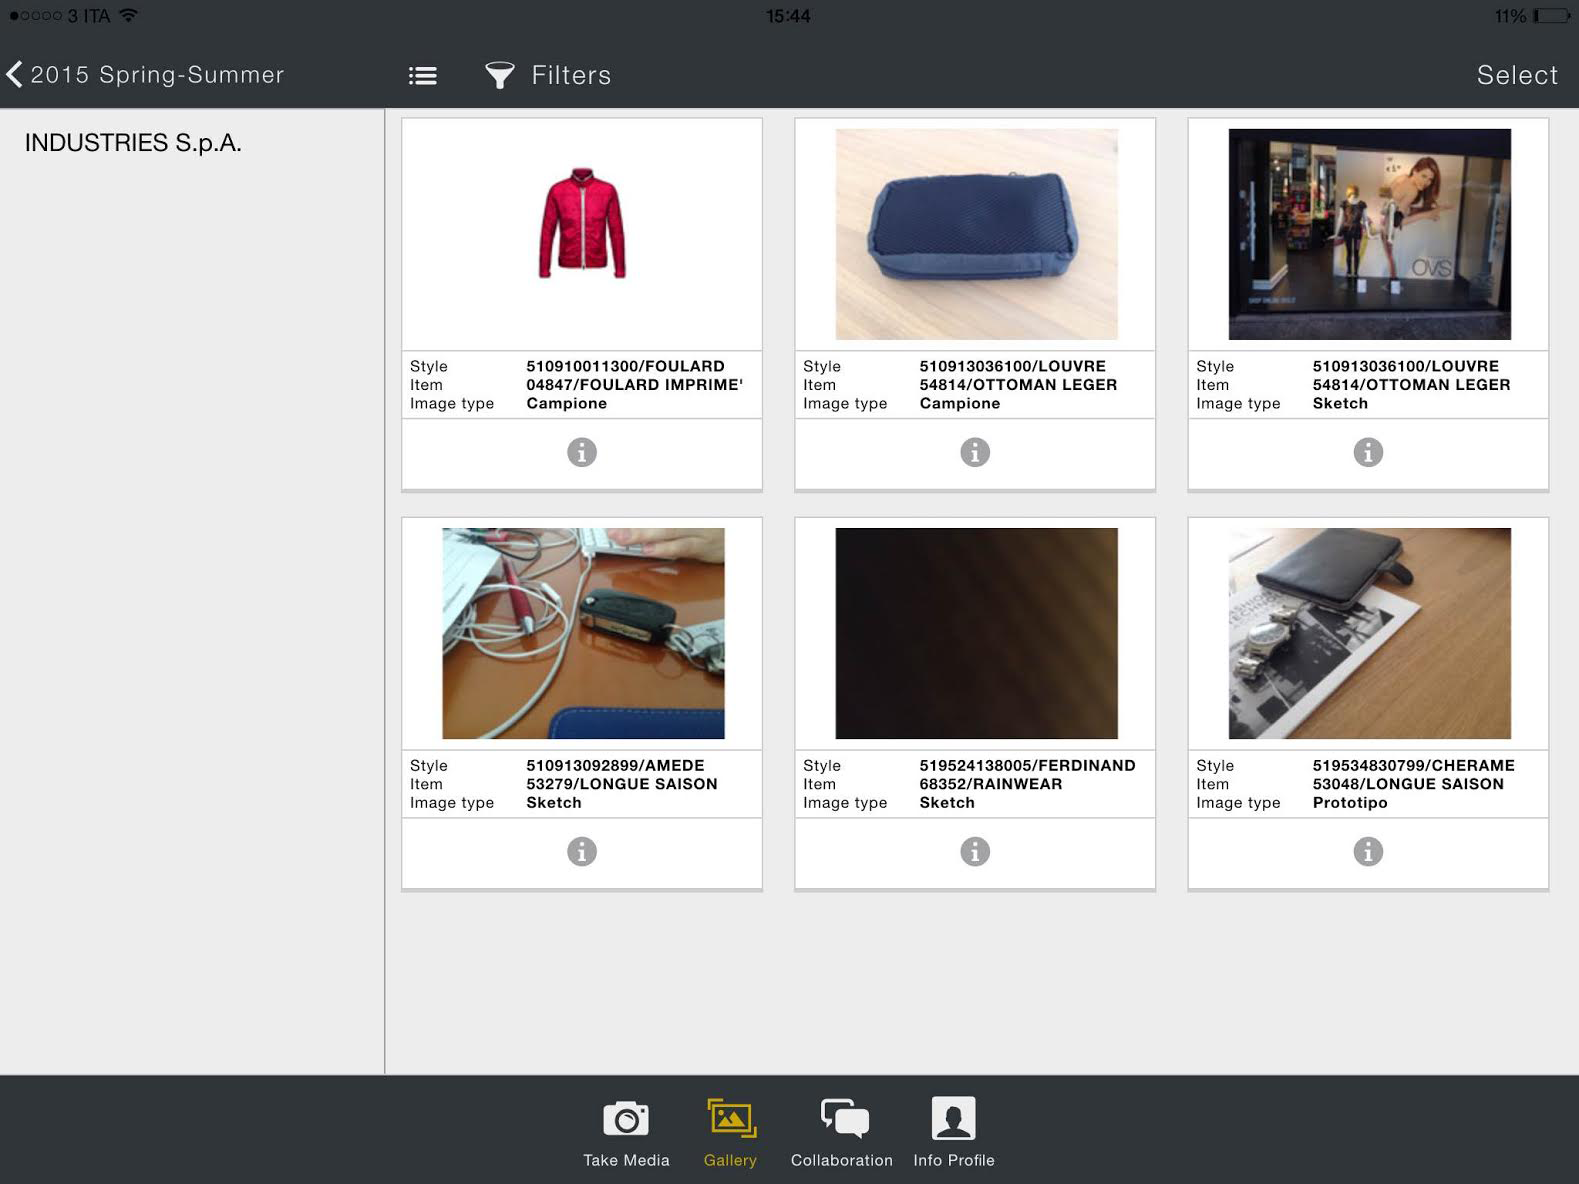
\includegraphics[width=\textwidth]{../immagini/warda-gallery}
\caption{Screenshot della gallery dell'applicazione attuale}  
\end{figure}

\subsubsection{Lista dei nodi}

\todo[inline]{AskAlberto: Immagine della lista dei nodi, dove si vede più di qualche nodo }

La lista dei figli del nodo corrente visualizza il titolo di ogni nodo e, quando l'utente seleziona un nodo dalla lista, questa viene aggiornata in modo che visualizzi i nodi figli del nodo selezionato. 
La selezione di un nodo dalla lista comporta anche l'aggiornamento della griglia degli assets, la quale andrà a visualizzare gli assets contenuti nel nodo selezionato.

Durante il caricamento dei dati della lista viene visualizzato un indicatore di attività per fornire all'utente un feedback riguardo l'operazione di caricamento dei dati in corso.

Sopra la lista dei nodi è presente un pulsante che permette di tornare al nodo padre del nodo correntemente visualizzato.

Questo pulsante è caratterizzato da una freccia indietro e dal titolo del nodo correntemente visualizzato, nel caso il nodo corrente sia il nodo radice della gallery, il pulsante non deve essere visibile.

\subsubsection{Griglia degli assets}

\begin{figure}[htp]
\centering
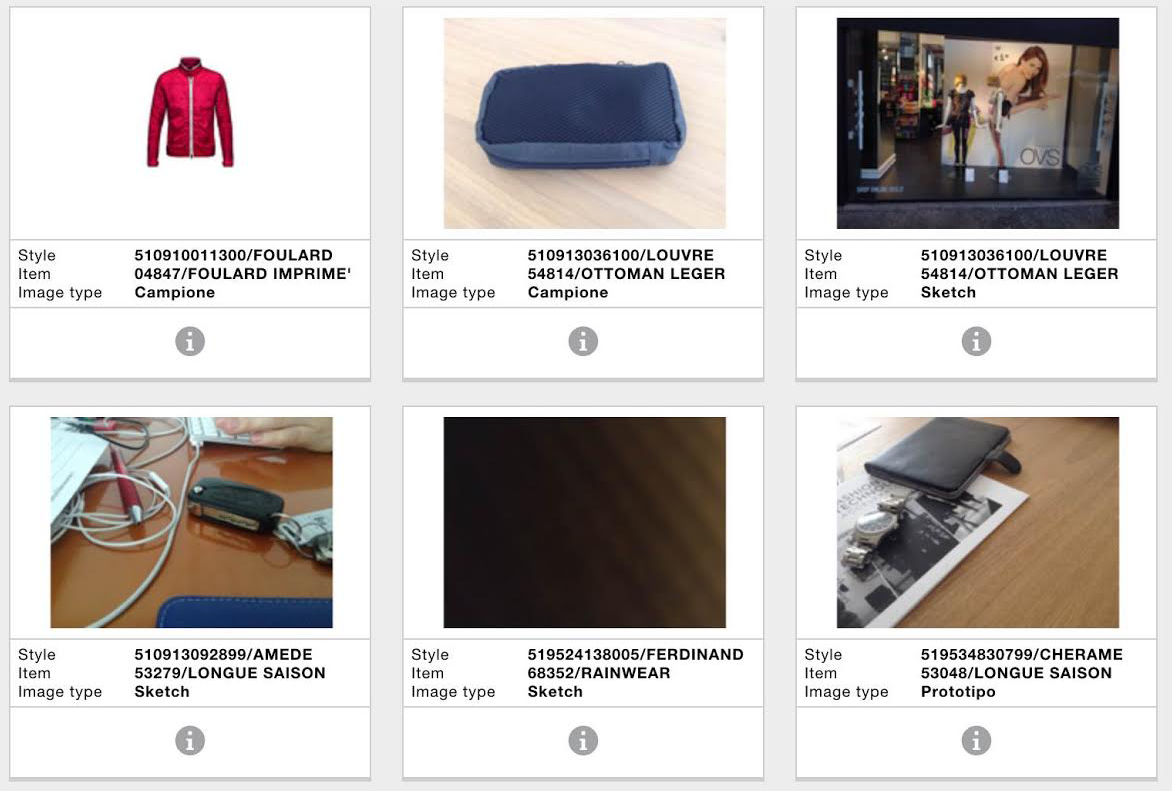
\includegraphics[width=\textwidth]{../immagini/warda-gallery-griglia}
\caption{Dettaglio della griglia degli assets dell'applicazione attuale}  
\end{figure}

La griglia degli assets rappresenta il componente principale dell'applicazione, questa griglia permette di visualizzare, per ogni asset contenuto nel nodo corrente, un'immagine di anteprima e un pulsante che permette all'utente di visualizzare i dettagli dell'asset mediante un \gls{popover}.

\begin{figure}[htp]
\centering
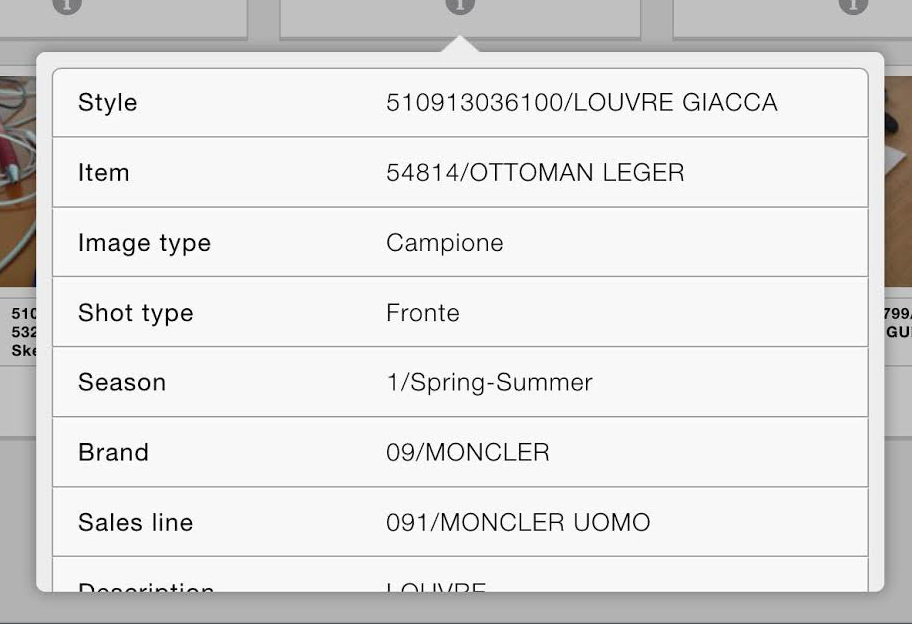
\includegraphics[width=\textwidth*3/4]{../immagini/warda-gallery-dettaglio}
\caption{Popover che mostra i dettagli di un asset}  
\end{figure}

Se l'utente esegue un \gls{tap} sull'immagine di un asset, viene visualizzata una pagina dell'applicazione contenente i dettagli dell'asset e un'immagine ingrandita, maggiori informazioni riguardo questa pagina sono disponibili nella sezione §\ref{sec:pag-dettaglio-asset}.

\todo[inline]{AskAlberto: Quanti assets vengono caricati per volta dalla griglia?}

Per motivi prestazionali, la griglia non carica subito tutti gli assets contenuti nel nodo corrente ma si limita a visualizzare solo i primi 25 assets, i successivi assets contenuti nel nodo vengono caricati man mano che l'utente prosegue nella visualizzazione della griglia, secondo il sistema dello scroll infinito.

\subsubsection{Lista dei filtri}

\todo[inline]{AskAlberto: Immagine della lista dei filtri}
La lista dei filtri compare come popovrt quando l'utente esegue un tap sul pulsante ``Filters'' presente nella barra di navigazione.

Per ogni filtro presente nel nodo corrente, viene visualizzata una lista dei possibili valori che possono essere assegnati al filtro ed una casella di testo che permette all'utente di filtrare i valori presenti nella lista.

\subsection{Pagina di dettaglio di un asset}\label{sec:pag-dettaglio-asset}

Questa pagina contiene l'immagine ingrandita di un asset e una lista con tutti i dettagli dell'asset.

Mediante un apposito pulsante l'utente può nascondere o rendere visibile la lista dei dettagli, in modo da lasciare più spazio all'immagine.

Sull'immagine l'utente può eseguire alcune gesture:
\begin{itemize}
\item \gls{swipe} verso sinistra, per visualizzare l'asset successivo contenuto nel nodo visualizzato dalla gallery;
\item swipe verso destra, per visualizzare l'asset precedente contenuto nel nodo visualizzato dalla gallery;
\item pinch-to-zoom, per ingrandire ulteriormente l'immagine.
\end{itemize}

Infine, nella barra di navigazione della pagina è presente un pulsante che permette all'utente di tornare alla pagina con la visualizzazione a griglia.

\todo[inline]{AskAlberto: immagine della visualizzazione di dettaglio, sia con la sidenav aperta, sia con la sidenav chiusa}

\section{Requisiti individuati}

I requisiti individuati dall'analisi dell'applicazione attuale e dalle discussioni con il tutor aziendale sono stati catalogati secondo il codice:
\begin{center}
\textit{R[T][I][C]}
\end{center}
dove:
\begin{itemize}
\item \textbf{T}ipo: specifica la tipologia del requisito e può assumere i seguenti valori:
	\begin{itemize}
	\item \textbf{F} - \textit{funzionale}, cioè che determina una funzionalità dell'applicazione;
	\item \textbf{V} - \textit{vincolo}, che riguarda un vincolo che il prodotto deve rispettare.
	\end{itemize}
\item \textbf{I}mportanza: specifica l'importanza del requisito e può assumere i seguenti valori:
	\begin{itemize}
	\item \textbf{O} - \textit{obbligatorio}, il requisito corrisponde ad un obbiettivo minimo del piano di stage e deve essere soddisfatto per garantire il funzionamento minimo dell'applicazione;
	\item \textbf{D} - \textit{desiderabile}, il requisito corrisponde ad un obbiettivo massimo del piano di stage e deve essere soddisfatto per garantire il funzionamento dell'applicazione;
	\item \textbf{F} - \textit{facoltativo}, indica che il requisito fornisce del valore aggiunto all'applicazione e non era stato previsto nel piano di stage.
	\end{itemize}
\item \textbf{C}odice: rappresenta un codice che identifica il requisito all'interno di una gerarchia. Questo codice è definito in modo che il il requisito \textit{RTIx.y} sia un requisito che va a definire con un grado maggiore di dettaglio alcuni degli aspetti del requisito \textit{RTIx}.
\end{itemize}


%subsection
\subsection{Requisiti Funzionali}
\normalsize
\begin{longtable}{|c|m{10cm}|}
\hline
\textbf{Id Requisito} & \textbf{Descrizione}\\
\hline
\endhead
RFO1 & L'utente deve poter visualizzare una gallery dell'applicazione WARDA a partire dal nodo radice della gallery \\ \hline
RFO1.1 & L'utente deve poter visualizzare la lista dei nodi contenuti nel nodo correntemente visualizzato \\ \hline
RFD1.1.1 & Durante il caricamento della lista dei nodi, deve essere presente un indicatore di attività per evidenziare l'attività in corso \\ \hline
RFD1.2 & L'utente deve poter rendere visibile la lista dei nodi contenuti nel nodo corrente \\ \hline
RFF1.2.1 & La comparsa della lista dei nodi deve avvenire in modo animato \\ \hline
RFD1.3 & L'utente deve poter nascondere la lista dei nodi dei nodi contenuti nel nodo corrente \\ \hline
RFF1.3.1 & La scomparsa della lista dei nodi deve avvenire in modo animato \\ \hline
RFO1.4 & L'utente deve poter spostarsi tra i nodi presenti in una gallery \\ \hline
RFO1.4.1 & L'utente deve poter selezionare un nodo contenuto nel nodo corrente per visualizzarne i contenuti \\ \hline
RFO1.4.2 & L'utente deve poter ritornare al nodo precedente visualizzato \\ \hline
RFF1.4.3 & Il cambiamento degli elementi presente nella lista dei nodi deve essere animato \\ \hline
RFO1.4.4 & Lo spostamento da un nodo all'altro deve comportare l'aggiornamento della lista dei nodi figli e della lista degli assets \\ \hline
RFO1.5 & L'utente deve poter visualizzare la lista degli assets contenuti nel nodo correntemente visualizzato \\ \hline
RFD1.5.1 & Durante il caricamento degli elementi della lista, deve essere presente un indicatore di attività per evidenziare l'attività in corso \\ \hline
RFO1.5.2 & La lista contenente gli assets deve avere un layout a griglia \\ \hline
RFO1.5.3 & La lista deve visualizzare un numero limitato di assets ed essere dotata di un sistema di scroll infinito \\ \hline
RFO1.5.3.1 & Una volta che l'utente visualizza tutti gli assets contenuti della griglia, se presenti, devono essere caricati ulteriori assets \\ \hline
RFO1.5.3.2 & Durante il caricamento degli ulteriori assets deve essere presente un indicatore di attività \\ \hline
RFO1.5.4. & Gli elementi della lista degli assets devono essere composti da un'immagine di anteprima dell'asset e da un pulsante ``Info'' \\ \hline
RFO1.5.4.1 & Quando l'utente esegue un tap sull'immagine di anteprima di un asset, deve essere visualizzata la pagina di dettaglio dell'asset \\ \hline
RFO1.5.4.2 & Quando l'utente esegue un tap sul pulsante Info di un asset, deve essere visualizzato un popover contenente le informazioni di dettaglio dell'asset \\ \hline
RFO1.6 & L'utente deve poter visualizzare la lista dei filtri disponibili per il nodo correntemente visualizzato \\ \hline
RFO1.6.1 & Per ogni filtro disponibile, l'utente deve poter visualizzare tutti i valori che può assumere il filtro \\ \hline
RFD1.6.1.1 & L'utente deve poter cercare un determinato valore all'interno della lista dei valori che può assumere il filtro \\ \hline
RFO1.6.1.2 & L'utente deve poter selezionare un valore per il filtro da applicare \\ \hline
RFO1.6.2 & L'utente deve poter applicare più filtri contemporaneamente \\ \hline
RFO1.6.3 & L'utente deve poter rimuovre un filtro \\ \hline
RFO1.6.4 & L'utente deve poter rimuovere tutti i filtri applicati \\ \hline
RFD1.6.5 & L'utente deve poter visualizzare il numero di filtri applicati \\ \hline
RFO1.6.6 & I filitri devono rimanere attivi anche se l'utente si sposta su un altro nodo \\ \hline
RFD1.6.7 & La lista dei filtri deve essere visualizzata come un pop-up \\ \hline
RFO2 & L'utente deve poter visualizzare una pagina contenente i dettagli di un asset \\ \hline
RFO2.1 & L'utente deve poter tornare alla pagina contenente la gallery \\ \hline
RFO2.2 & L'utente deve poter visualizzare un'immagine ingrandita dell'asset \\ \hline
RFD2.2.1 & Durante il caricamento dell'immagine, deve essere presente un indicatore di attività che visualizzi la percentuale di caricamento \\ \hline
RFF2.2.2 & L'utente deve poter effettuare il pinch-to-zoom sull'immagine \\ \hline
RFO2.2.3 & L'utente deve poter effettuare uno swipe da destra verso sinistra sull'immagine, per visualizzare in dettaglio l'asset successivo secondo l'ordine del contenuto della gallery \\ \hline
RFF2.2.3.1 & Allo swipe deve essere associata un'animazione che sposti l'immagine da destra verso sinistra seguendo il movimento effettuato dall'utente \\ \hline
RFF2.2.3.2 & Nel caso non sia presente un'asset successivo da visualizzare, l'animazione dello swipe deve essere interrotta \\ \hline
RFO2.2.4 & L'utente deve poter effettuare uno swipe da sinistra verso destra sull'immagine, per visualizzare in dettaglio l'asset precedente secondo l'ordine del contenuto della gallery \\ \hline
RFF2.2.4.1 & Allo swipe deve essere associata un'animazione che sposti l'immagine da sinistra verso destro seguendo il movimento effettuato dall'utente \\ \hline
RFF2.2.4.2 & Nel caso non sia presente un'asset precedente da visualizzare, l'animazione dello swipe deve essere interrotta \\ \hline
RDO2.3 & L'utente deve poter visualizzare una lista contenente i dettagli dell'asset visualizzato \\ \hline
RFD2.4 & L'utente deve poter rendere visibile la lista contenente i dettagli dell'asset visualizzato \\ \hline
RFF2.4.1 & La comparsa della lista contenente i dettagli deve avvenire in modo animato \\ \hline
RFD2.5 & L'utente deve poter nascondere la lista contenente i dettagli dell'asset visualizzato \\ \hline
RFF2.4.1 & La scomparsa della lista contenente i dettagli deve avvenire in modo animato \\ \hline
RFF3 & L'utente deve visualizzare un messaggio d'errore nel caso l'applicazione non riesca a connettersi con il server \\ \hline
\caption[Requisiti Funzionali]{Requisiti Funzionali}
\label{tabella:req0}
\end{longtable}

\subsection{Requisiti di Vincolo}
\normalsize
\begin{longtable}{|c|m{10cm}|}
\hline
\textbf{Id Requisito} & \textbf{Descrizione} \\
\hline
\endhead
RVD1 & L'applicazione deve essere dotata di un file di configurazione che permette di impostare: l'indirizzo del server a cui connettersi, l'id della gallery da visualizzare, l'username e password con i dati da utilizzare per effettuare l'accesso e il numero di assets da visualizzare in una singola pagina \\ \hline
RVO2 & L'applicazione deve essere realizzata con React Native \\ \hline
RVO3 & L'applicazione deve essere compatibile con iPad di seconda generazione \\ \hline
RVD4 & L'interfaccia grafica dell'applicazione deve essere fluida e non bloccarsi \\ \hline
\caption[Requisiti di Vincolo]{Requisiti di Vincolo}
\label{tabella:req1}
\end{longtable}



\section{Riepilogo requisiti}

In totale sono stati individuati 52 requisiti, ripartiti tra le varie tipologie secondo quanto riportato nelle seguenti tabelle.
\\ \\ \\
\begin{minipage}{\textwidth}
  \begin{minipage}[b]{0.49\textwidth}
    \centering
      \begin{tabular}{|l|c|} \hline
      \textbf{Importanza} & \textbf{\#} \\ \hline
  Obbligatori & 29 \\ \hline
  Desiderabili & 12 \\ \hline
  Facoltativi & 11 \\ \hline
  Totale & 52 \\ \hline
\end{tabular}
      \captionof{table}{Numero di requisiti per importanza}
	\end{minipage}
	  \hfill
  \begin{minipage}[b]{0.49\textwidth}
    \centering
         \begin{tabular}{|l|c|} \hline
      \textbf{Tipologia} & \textbf{\#} \\ \hline
  Funzionali & 48 \\ \hline
  Vincolo & 4 \\ \hline
    Totale & 52 \\ \hline
\end{tabular}
    \captionof{table}{Numero di requisiti per tipologia}
  \end{minipage}
\end{minipage}
 \\ \\ \\

\begin{minipage}{\textwidth}
  \begin{minipage}[b]{0.49\textwidth}
    \centering
    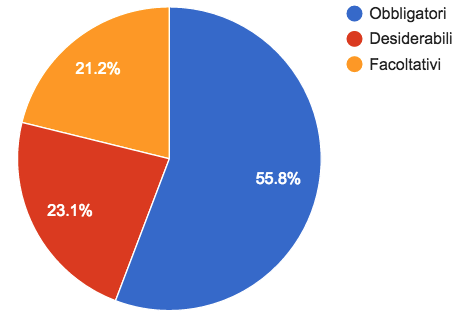
\includegraphics[scale=0.7]{../immagini/requisiti-totale-importanza}
      \captionof{figure}{Requisiti per importanza}
	\end{minipage}
	  \hfill
  \begin{minipage}[b]{0.49\textwidth}
    \centering
  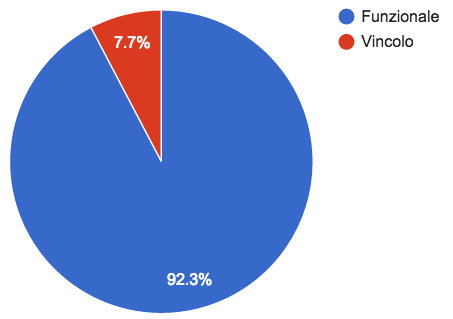
\includegraphics[scale=0.7]{../immagini/requisiti-totale-tipologia}
      \captionof{figure}{Requisiti per tipologia}
  \end{minipage}
\end{minipage}



